% !TEX root =  ../../../thesis.tex
\section{Image Features}\label{sec:aam:features}
A feature-based image representation is achieved with the application of a
feature extraction function, as defined in Eq.~\ref{equ:feature_function}. In this work, we require the descriptor function to extract densely-sampled image features, thus compute a feature vector for each pixel location. Given an input image of size $H\times W$ in vectorial form $\mathbf{t}$ with length $L_T=HW$,
the descriptor-based image vector is
%%%%%%%%%%%%%%
\begin{equation}
  \mathbf{f} = \mathcal{F}(\mathbf{t})
  \label{equ:featuresFunction}
\end{equation}
%%%%%%%%%%%%%%
with size $L_TD\times 1$, where $D$ is the number of channels.
In the rest of the chapter, we will denote the images in vectorized form within
the equations.

Many robust multi-dimensional image descriptors have been proposed and applied
to various tasks. They can be divided in two categories: those extracted based
only on the pixel values and those extracted based on larger spatial
neighborhoods. They all aim to generate features that are invariant to
translation, rotation, scale and illumination changes and robust to local
geometric distortion. We select nine of the most powerful and successful
descriptors, which are briefly described in the following subsections
(\ref{sec:aam:features:gradeintOrientation}--\ref{sec:aam:features:gabor}).
Figure~\ref{fig:featuresImages} shows the feature-based image representation
for each of the employed feature types. The visualized grayscale images are
constructed by summing all the $D$ channels of the feature images. Notice how
each descriptor handles the illumination changes and the face's distinctive
edges. Table~\ref{tab:featuresParameters} summarizes the parameter values, the
number of channels and the neighborhood size that gets involved in computing
the descriptor at each image location for all features.

% Edge Structure
\subsection{Edge Structure (ES)}\label{sec:aam:features:gradeintOrientation}
ES, initially proposed in~\cite{cootes2001representing}, is a measure which
captures the orientation of image structure at each pixel, together with an
indication of how accurate the orientation estimate is. The accuracy belief
measure penalizes the orientations in flat, noisy regions and favors the ones
near strong edges. The first step of the ES features computation involves the
estimation of the local gradients with respect to $x$ and $y$, denoted by
$\mathbf{g}_x$ and $\mathbf{g}_y$, and the calculation of the gradient
magnitude $\mathbf{g}=\sqrt{\mathbf{g}_x^2+\mathbf{g}_y^2}$. Then
$\mathbf{f}=f(\mathbf{g})[\mathbf{g}_x,\mathbf{g}_y]$ is evaluated, where
$f(\mathbf{g})=|\mathbf{g}|/(|\mathbf{g}|+\bar{g})$ is a non-linear
normalization function ($\bar{g}$ is the mean of $\mathbf{g}$). This
feature-based representation has $D=2$ channels and is effective at favoring
strong and distinctive edges (Fig.~\ref{fig_feat:es}).

% Features Image Examples
\begin{figure}[!t]
\centering
\subfloat[Original]{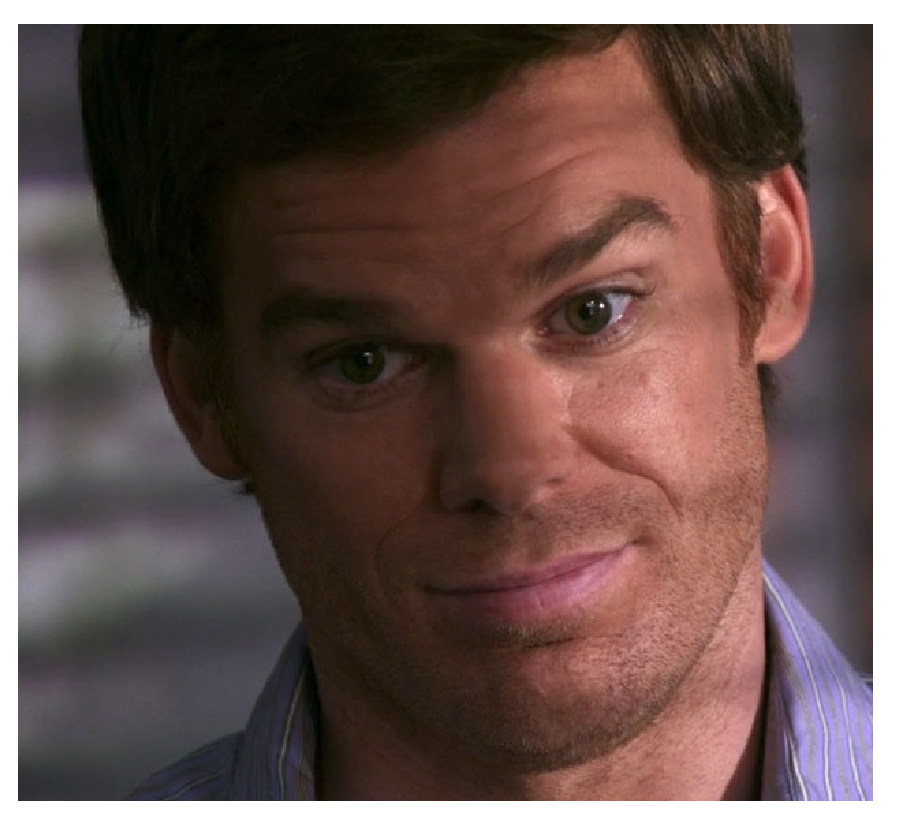
\includegraphics[width=0.2\linewidth]{figures/feature_based_aam/1_FeaturesImages/original}\label{fig_feat:original}}
\subfloat[ES]{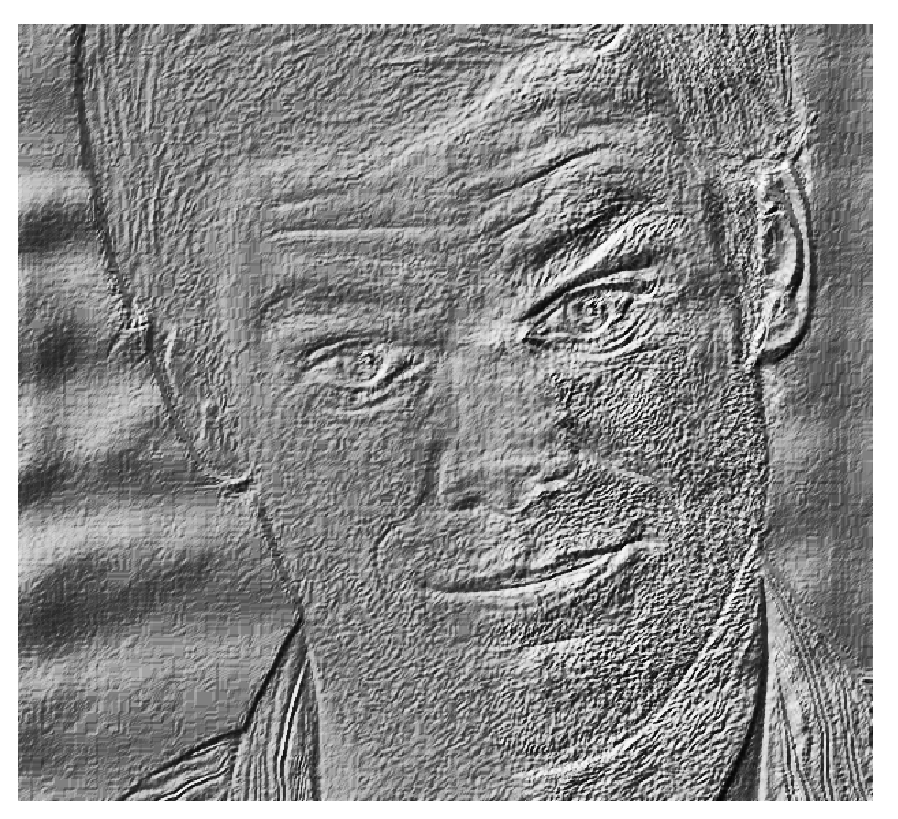
\includegraphics[width=0.2\linewidth]{figures/feature_based_aam/1_FeaturesImages/go}\label{fig_feat:es}}
\subfloat[IGO]{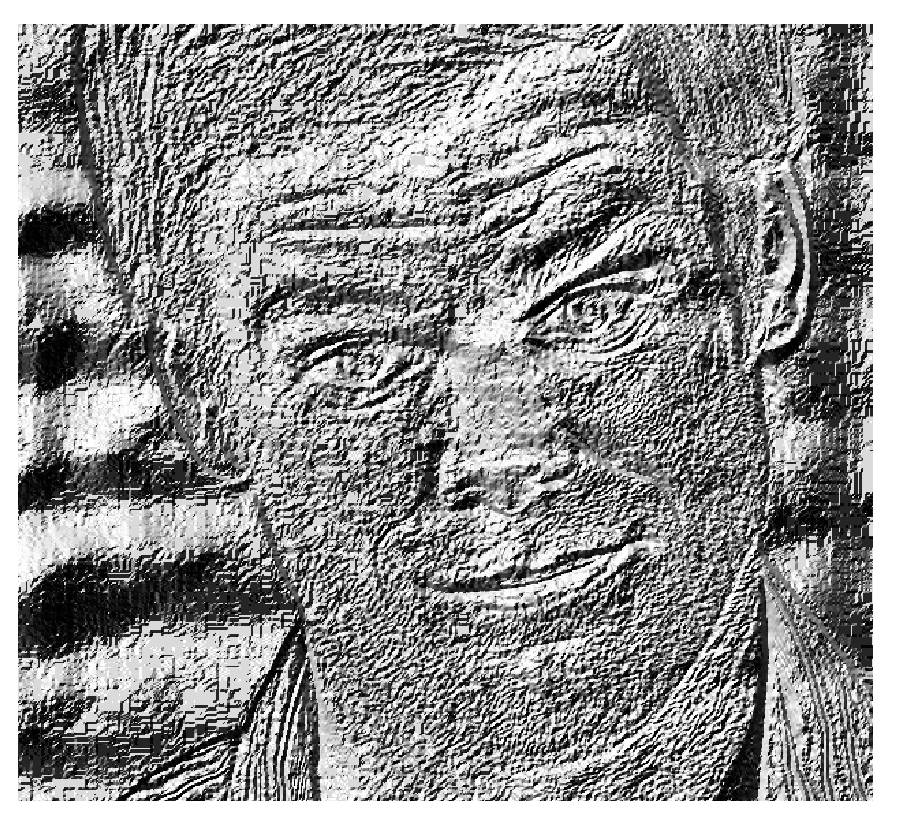
\includegraphics[width=0.2\linewidth]{figures/feature_based_aam/1_FeaturesImages/igo}\label{fig_feat:igo}}
\subfloat[HOG]{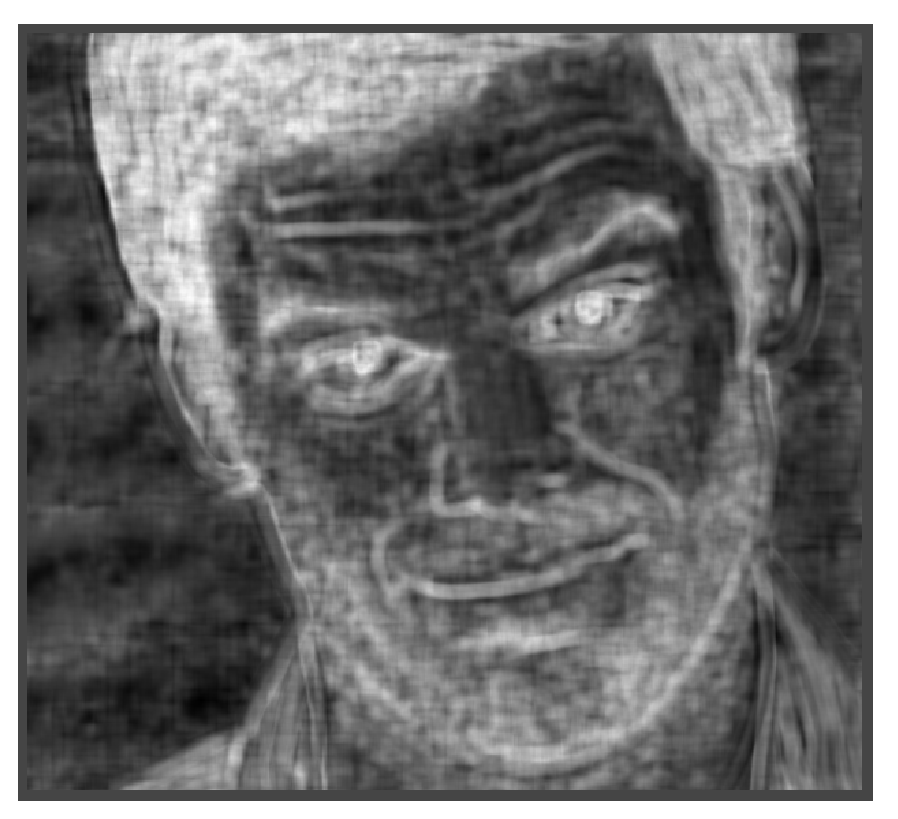
\includegraphics[width=0.2\linewidth]{figures/feature_based_aam/1_FeaturesImages/hog}\label{fig_feat:hog}}
\subfloat[SIFT]{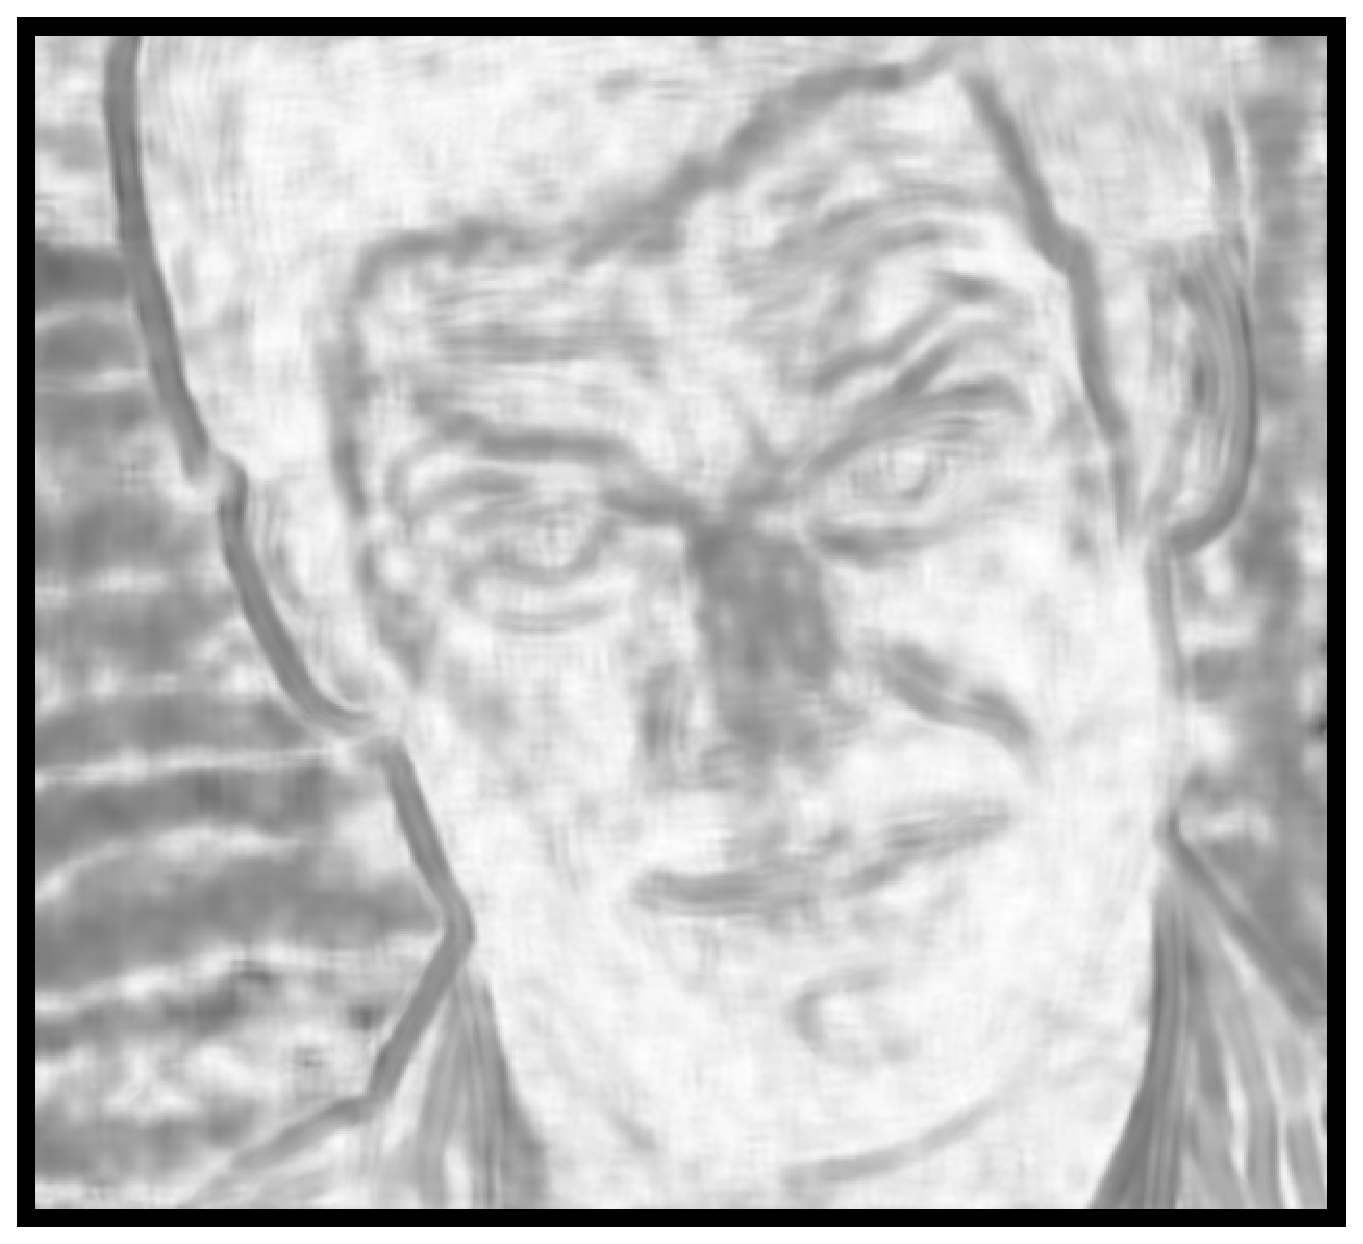
\includegraphics[width=0.2\linewidth]{figures/feature_based_aam/1_FeaturesImages/sift}\label{fig_feat:sift}}\\
\subfloat[OLBP]{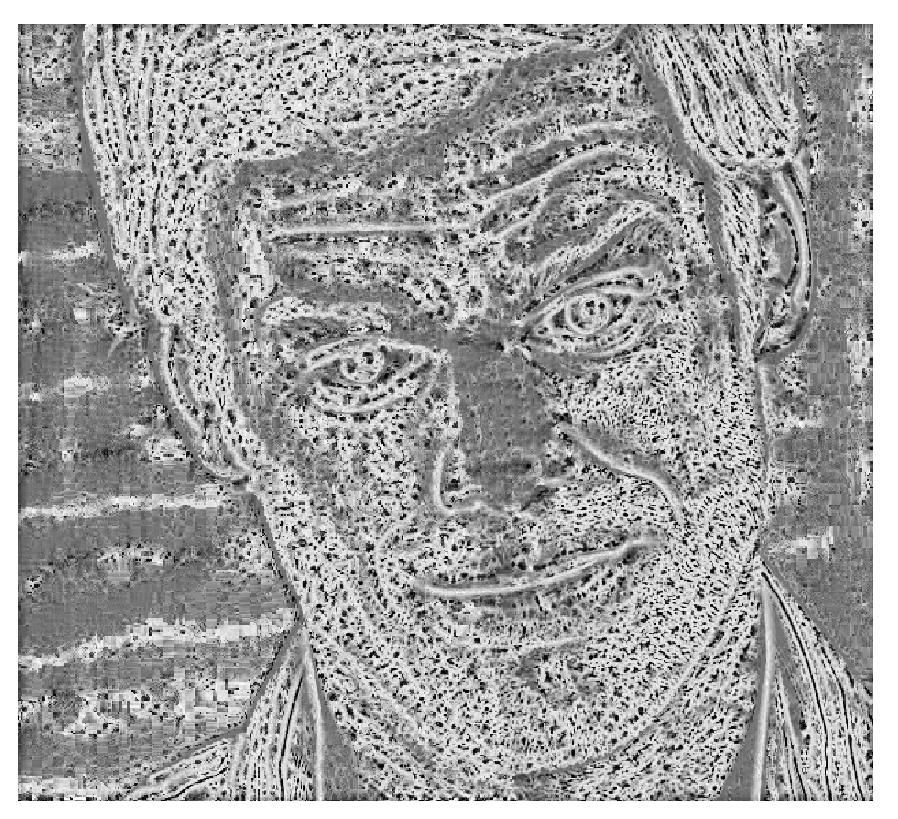
\includegraphics[width=0.2\linewidth]{figures/feature_based_aam/1_FeaturesImages/olbp}\label{fig_feat:olbp}}
\subfloat[TPLBP]{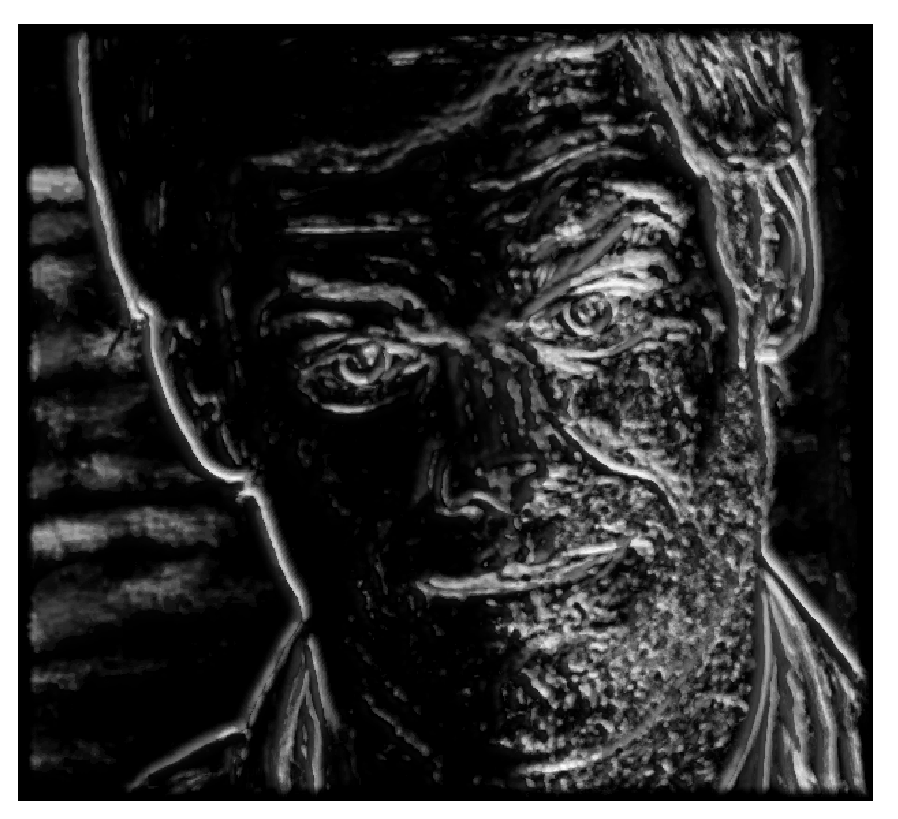
\includegraphics[width=0.2\linewidth]{figures/feature_based_aam/1_FeaturesImages/tplbp}\label{fig_feat:tplbp}}
\subfloat[FPLBP]{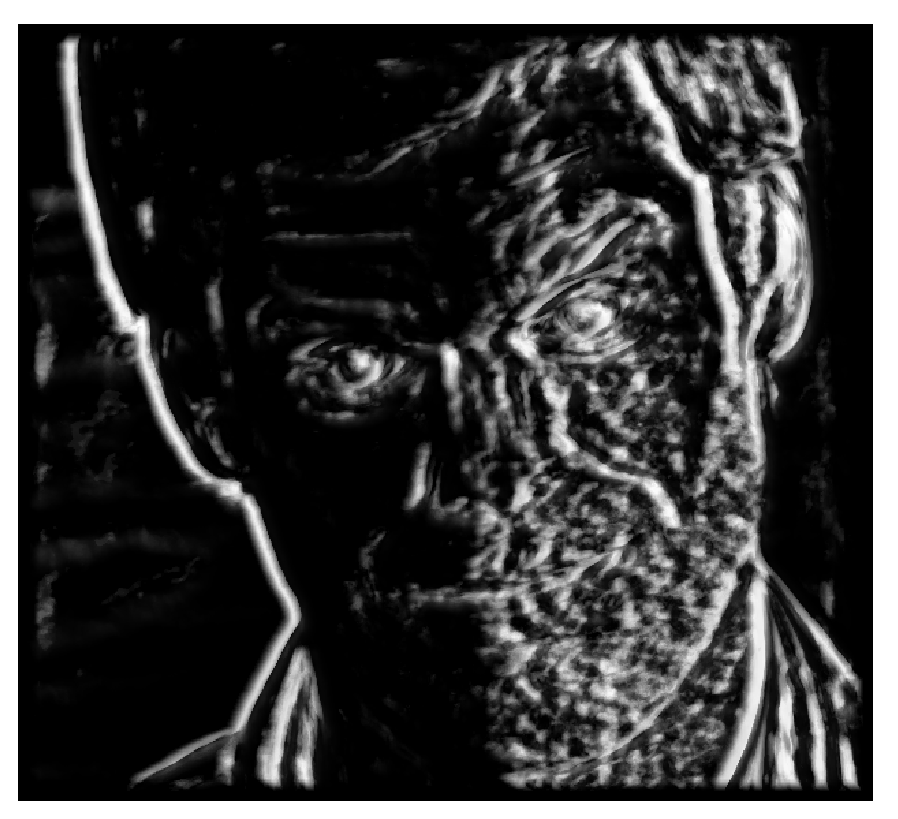
\includegraphics[width=0.2\linewidth]{figures/feature_based_aam/1_FeaturesImages/fplbp}\label{fig_feat:fplbp}}
\subfloat[Gabor Angles]{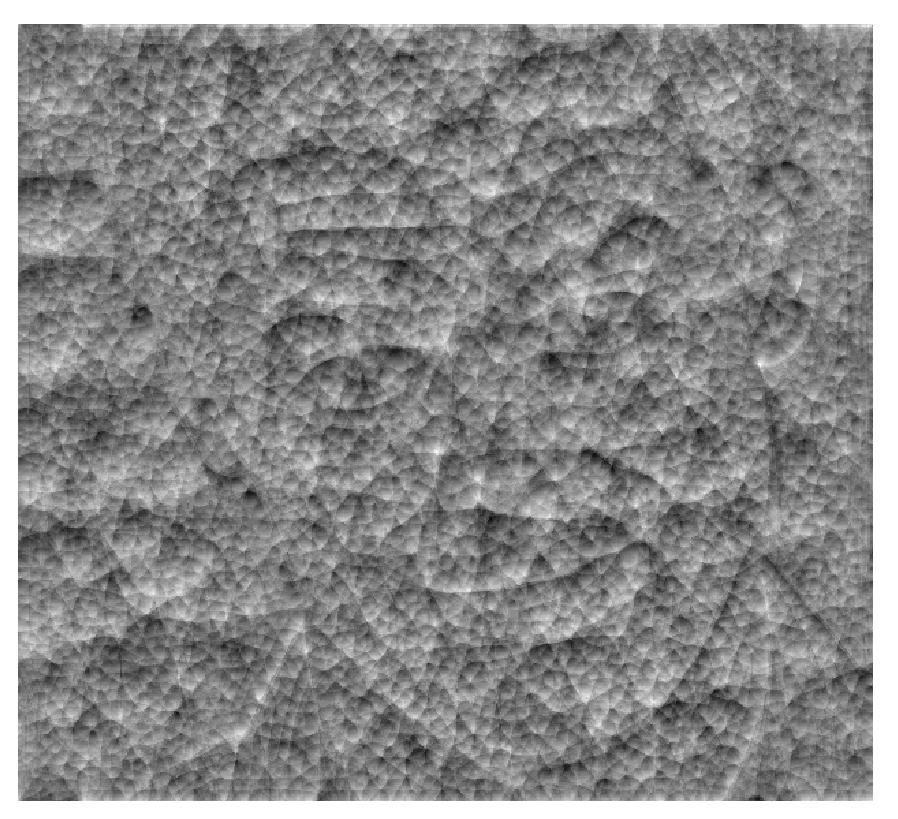
\includegraphics[width=0.2\linewidth]{figures/feature_based_aam/1_FeaturesImages/gabor_angles}\label{fig_feat:gabor_angles}}
\subfloat[Gabor Magnitude]{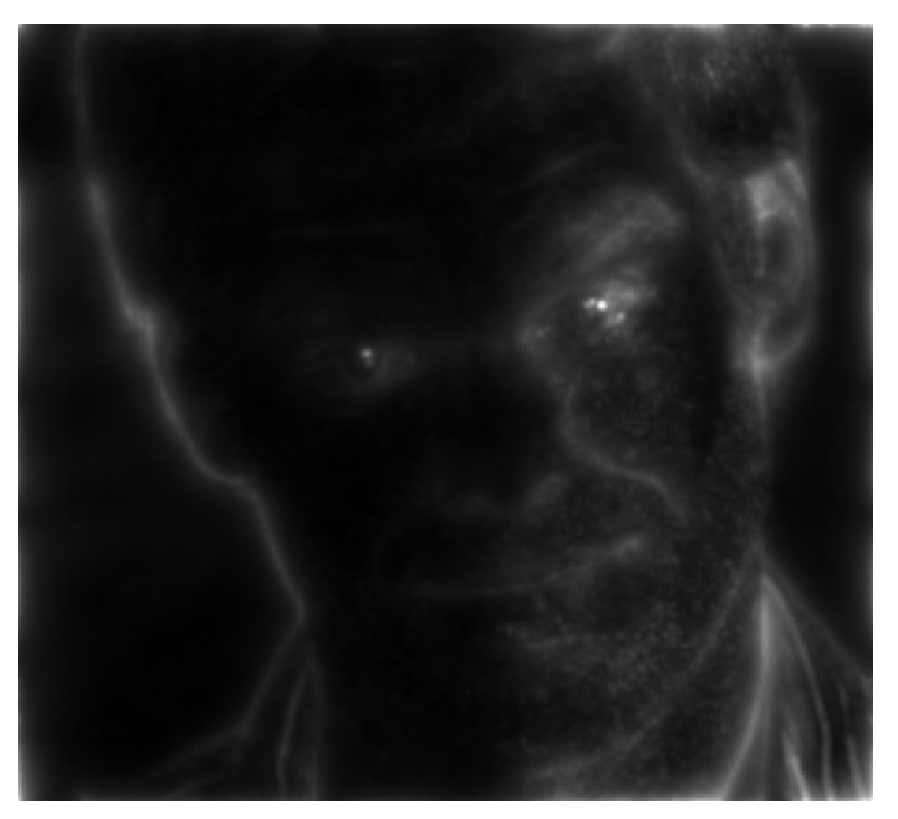
\includegraphics[width=0.2\linewidth]{figures/feature_based_aam/1_FeaturesImages/gabor_magnitude}\label{fig_feat:gabor_magnitude}}
\caption{Examples of the nine employed dense feature types. The feature images
have the same height and width as the original image and $D$ channels.
In order to visualize them, we compute the sum over all $D$ channels.}
\label{fig:featuresImages}
\end{figure}
%

% IGO
\subsection{Image Gradient Orientation (IGO)}
\label{sec:aam:features:gradeintCorrelation}
IGO is introduced and successfully applied
in~\cite{tzimiropoulos2012generic,tzimiropoulos2011robust,tzimiropoulos2012subspace,tzimiropoulos2014active}.
Given the gradients $\mathbf{g}_x$, $\mathbf{g}_y$ of an input image and their
orientation $\boldsymbol{\varphi}$, we compute the IGO image as
$\mathbf{f} = \frac{1}{\sqrt{L_T}} [\cos{\boldsymbol{\varphi}}^\mathsf{T}, ~\sin{\boldsymbol{\varphi}}^\mathsf{T}]^\mathsf{T}$,
where $L_T$ is the length of the input image and
$\cos{\boldsymbol{\varphi}} = \left[\cos{\boldsymbol{\varphi}(1)}, \ldots, \cos{\boldsymbol{\varphi}(L_T)}\right]^\mathsf{T}$
(the same for $\sin{\boldsymbol{\varphi}}$). The above feature image definition
results in $D=2$ channels. IGO features allow us to estimate the similarity
between two images as $s=\mathbf{f}_1^\mathsf{T}\mathbf{f}_2$. This measure
becomes $s\approx0$ for the image areas that are corrupted by outliers (e.g.
occlusion) and thus behaves similarly to weighted least-squares kernel without
the need of information regarding the structure of outliers. This reveals the
advantage of this feature. IGO is robust to outliers while at the same time
being low-dimensional compared to other robust features
(Fig.~\ref{fig_feat:igo}).

% HOG
\subsection{Histograms of Oriented Gradients (HOG)}
\label{sec:aam:features:hog}
HOG descriptors~\cite{dalal2005histograms} cluster the gradient orientations in
different bins for localized sub-windows of an input image resulting in
counting occurrences of the orientations. Thus, the shape and texture of the
image are described by histograms of local edge directions, which are also
characterized by photometric invariance. The HOG features extraction begins by
computing the image gradient. If the image is color, then the gradient with the
largest norm between the three channels is kept. Two spatial neighborhoods are
used at the region of each pixel: cells and blocks. A cell is a small
sub-window from which we create a histogram of the gradient's orientations
weighted by the gradient magnitude. The histogram has $N_{bins}$ bins and
trilinear interpolation is applied between the votes of neighboring bin centers
with respect to orientation and position. A block is a larger spatial region
that consists of $N_{block}\times N_{block}$ cells. We apply contrast
normalization between the cells that are grouped within a block, based on the
Euclidean norm. The final descriptor vector extracted from each block is
composed by concatenating the normalized histograms of the cells, thus it has
length $D=N_{bins}N^2_{block}$. In the default HOG formulation, the block can
be regarded as a sliding window that scans the locations of an image with a
sampling step of either a block (no overlap) or half a block (overlapping
windows). On the contrary, the computed feature image in our case is dense,
which means that we use a sampling step of one pixel and we extract a
descriptor vector from the block centered at each such location. This ends up
in a very powerful representation that is descriptive on the important facial
parts and flat on the rest of the face (Fig.~\ref{fig_feat:hog}). By using
cells of size $8\times8$ pixels with $N_{block}=2$ and $N_{bins}=9$,
we have $D=36$ channels.

% SIFT
\subsection{Scale-Invariant Feature Transform (SIFT)}
\label{sec:aam:features:sift}
SIFT features, originally proposed in~\cite{lowe1999object}, are computed
locally based on the appearance of particular interest points (keypoints). In
the original SIFT formulation, these keypoints are detected as the maxima and
minima of the Difference of Gaussians applied in the scale space of an image.
The scale space is constructed by convolving the image with Gaussian filters at
different scales (and octaves). The keypoints with dominant orientations are
kept and the points that have low contrast or lie along an edge are ignored.
Then SIFT descriptors are obtained by taking into account neighboring pixels
within a radius for a keypoint. Thus, the traditional SIFT framework returns a
sparse feature map of an image, which is not useful in our case. Similar to the
HOG case, in our framework, we skip the keypoint detection step and extract a
SIFT descriptor vector for each image location.

We begin by assigning a dominant orientation to each pixel. Assume that
$\mathbf{L}(x,y,\sigma)=\mathbf{G}(x,y,\sigma)\ast\mathbf{T}(x,y)$ is the
Gaussian-smoothed image at the scale $\sigma$ of the location $(x,y)$. We
calculate the gradient magnitude and direction for every pixel in a
neighborhood around the point in $\mathbf{L}$ and form an orientation
histogram, where each orientation is weighted by the corresponding gradient
magnitude and by a Gaussian-weighted circular window with standard deviation
proportional to the pixel's $\sigma$. Then, we take the orientations that are
within a percentage ($80\%$) of the highest bin. If these orientations are more
than one, then we create multiple points and assign them each orientation
value. Eventually, the final descriptor vector is created by sampling the
neighboring pixels at the image $\mathbf{L}(x,y,\sigma)$ with scale closest to
the point's scale, rotating the gradients and coordinates by the previously
computed dominant orientation, separating the neighborhood in
$N_{block}\times N_{block}$ sub-regions and create a Gaussian-weighted
orientations histogram for each sub-region with $N_{bins}$ bins. Finally, the
histograms are concatenated in a single vector with length
$D=N_{bins}N^2_{block}$ that is normalized to unit length. The SIFT descriptor
is similar to the HOG one, with the difference that the orientations histograms
are computed with respect to each point's dominant orientation. In general,
SIFT are invariant to scale, rotation, illumination and viewpoint
(Fig.~\ref{fig_feat:sift}). We use the same parameters as in HOGs
($N_{block}=2$, $N_{bins}=9$ and $8\times8$ cells), thus $D=36$ channels.

% LBP
\subsection{Local Binary Patterns (LBP)}\label{sec:aam:features:lbp}
The basic idea behind
LBP~\cite{ojala1996comparative,ojala2001generalized,ojala2002multiresolution}
is to encode the local structure in an image by comparing each pixel's
intensity value with the pixel intensities within its neighborhood. For each
pixel, we define a neighborhood radius $r$ centered at the pixel and compare
the intensities of $S$ circular sample points to its intensity. The sampling is
done clockwise or counter-clockwise, starting from a specific angle, and we
apply interpolation on sample points that are not discrete. If the center
pixel's intensity is greater or equal than the sample's, then we denote it by
$1$, otherwise by $0$. Thus, we end up with a binary number (LBP code) for each
pixel, with $S$ digits and $2^S$ possible combinations, which is converted to
decimal. In the original LBP formulation, the output is a descriptor vector
describing the whole image with a normalized histogram of the decimal codes. We
instead use $N_{radius}$ number of values for the radius parameter, $r$. Then
we sample $N_{samples}$ sets of points $S$ from the circle of each radius value
and concatenate the LBP codes in a vector. This means that our dense feature
image has $D=N_{radius}N_{samples}$ channels. We also employ the extension of
rotation-invariant uniform LBPs. Uniform LBPs are binary codes with at most two
circular $0$-$1$ and $1$-$0$ transitions. In the computation of the final LBP
patterns, there is a separate label for each uniform code and all the
non-uniform codes are labeled with a single label. By setting
$r=\{1,2,\ldots,8\}$ ($N_{radius}=8$) and sampling $N_{samples}=8$ points for
each radius value, we end up with $D=8$ channels.

Moreover, apart from the original LBP, which we denote by OLBP, we also use the
variations of Three-Patch LBP (TPLBP) and Four-Patch LBP (FPLBP), introduced
in~\cite{wolf2008descriptor}. TPLBP and FPLBP encode in the binary codes the
similarities between neighboring patches (for details, please refer
to~\cite{wolf2008descriptor}). Thus, the number of channels in this case also
depends on the employed number of patches $N_{patch}$ with different sizes,
hence $D=N_{radius}N_{samples}N_{patch}$. With the parameters we use, we end up
with $D=16$ channels. The three LBP derivatives are visualized in
Figs.~\ref{fig_feat:olbp}-\ref{fig_feat:fplbp}.

% Gabor
\subsection{Gabor Magnitude and Angle}\label{sec:aam:features:gabor}
Herein, we employ the log-Gabor filter
(wavelet)~\cite{kovesi1997symmetry,kovesi1999image,lee1996image}. In the
log-polar coordinates of the Fourier domain $(\rho,\theta)$, this is defined as
$G_{(s,o)}(\rho,\theta)=\allowbreak\exp{\left(-\frac{1}{2}\left(\frac{\rho-\rho_s}{\sigma_{\rho}}\right)^2\right)}\allowbreak\exp{\left(-\frac{1}{2}\left(\frac{\theta-\theta_{(s,o)}}{\sigma_{\theta}}\right)^2\right)}$,
where $\sigma_{\rho}$ and $\sigma_{\theta}$ are the bandwidths in $\rho$ and
$\theta$ respectively and $(s,o)$ are the indexes of each filter's scale and
orientation. Thus, by using $N_{sc}$ scales and $N_{or}$ orientations, we have
a filterbank of log-Gabor filters with $s=1,\ldots,N_{sc}$ and
$o=1,\ldots,N_{or}$. The reason why log-Gabor filter is preferred over Gabor is
that it has no DC component and its transfer function is extended at a high
frequency range. Given an image, we compute its convolution with each log-Gabor
filter for all scales and orientations. Then, we create two feature images by
concatenating the convolution's magnitude and phase, respectively. Both feature
versions have $D=N_{sc}N_{or}$ channels. An example of the Gabor angles and
magnitude is shown in Figs.~\ref{fig_feat:gabor_angles} and
\ref{fig_feat:gabor_magnitude}, respectively. We use the log-Gabor filters
implementation available in~\cite{kovesiMATLABCode} with $N_{sc}=4$ and
$N_{or}=9$, thus $D=36$.

% Features parameters, neighbourhood size and channels
\begin{table}[!t]
\renewcommand{\arraystretch}{1.3}
\centering
\begin{threeparttable}[b]
\begin{tabular}{c||c|c|c}
\multirow{2}{*}{\emph{Feature Type}} & \multirow{2}{*}{\emph{Parameters Values}} & \emph{Neighbourhood Size} & \multirow{2}{*}{\emph{Channels ($D$)}} \\
& & \emph{(in pixels)} & \\
\hline\hline
IGO, ES         & $-$                             & $-$                  & 2                   \\ \hline
HOG             & $N_{bins}=9$, $N_{cell}=2$      & \multirow{2}{*}{256} & \multirow{2}{*}{36} \\
SIFT            & $cell=8\times8~\text{pixels}$   &                      &                     \\ \hline
OLBP~\tnote{a}  & $N_{radius}=8$, $N_{samples}=8$ & 64                   & 8                   \\ \hline
TPLBP~\tnote{a} & $N_{radius}=8$, $N_{samples}=8$ & \multirow{2}{*}{64}  & \multirow{2}{*}{16} \\
FPLBP~\tnote{b} & $N_{patch}=2$                   &                      &                     \\ \hline
Gabor           & $N_{sc}=4$, $N_{or}=9$          & $-$                  & 36
\end{tabular}
\begin{tablenotes}
\item[a] Radius takes values $\{1,2,\ldots,8\}$, patch sizes are $2$ and $4$ and for each radius we sample a single set of $8$ points.
\item[b] Inner and outer radius are $\{[1,5],[2,6],\ldots,[8,12]\}$, patch sizes are $2$ and $4$ and for each radius we sample a single set of $8$ points.
\end{tablenotes}
\end{threeparttable}
\caption{Characteristics of the nine employed dense feature types. The characteristics include the features' parameters values, neighborhood size that contributes in each pixel's computation and number of channels.}
\label{tab:featuresParameters}
\end{table}
%

% Complexity
\subsection{Features Function Computational Complexity}
\label{sec:aam:features:complexity}
As mentioned before, the presented features can be separated in two categories:
\begin{enumerate}
  \item Features that are computed in a pixel-based fashion (\eg, ES, IGO).
  \item Features that are computed in a window-based mode, thus they depend on
  the values of a larger spatial neighborhood for each location (\eg, HOG,
  SIFT, LBP).
\end{enumerate}
Given an image $\mathbf{t}$ in vectorial form with length
$L_T$, the computational cost of extracting dense $D$-channel features of the
first category is $\mathcal{O}(L_TD)$. Respectively, the complexity of
extracting the features of the second category, using a window of size
$h\times w$ for each pixel, is $\mathcal{O}(L_TL_wD)$, where $L_w=hw$ is the
window's area. However, since the window's dimensions $h$ and $w$ take values
of the same order as $D$, hence $hw\approx D^2$, the cost of the second case
can also be expressed as
%%%%%%%%%%%%%%%%
\begin{equation}
\mathcal{O}(L_TD^3)
\label{equ:featuresCost}
\end{equation}
%%%%%%%%%%%%%%%%
This gives an intuition on the complexity difference between the two cases. In
the following sections, we will use the window-based features complexity of
Eq.\ref{equ:featuresCost} as the worst-case scenario, since it is more
expensive than the pixel-based one.
